%%%%%%%%%%%%%%%%%%%%%%%%%%%%%%%%%%%%%%%%%%%%%%%%%%%%%%%%
% Created by Pierre Chardaire. 
% Updated by Rudy Lapeer update: 10/2024
% Final Update by Mohsin Raza Last update: 10/2025
% Change the option between square brackets
% depending on the document you have to write:
%
% review      for the literature review + plan
% progress    for the progress report
% final       for the final report
% 
%%%%%%%%%%%%%%%%%%%%%%%%%%%%%%%%%%%%%%%%%%%%%%%%%%%%%%%%
\documentclass[progress]{cmpreport}


% Some package I am using. You may not need them
%
\usepackage{rotating}
\usepackage{subfloat}
\usepackage{color}
\usepackage{pdfpages}
\usepackage{amsmath}
\usepackage{enumitem}
\usepackage{booktabs}
\usepackage{graphicx}
\usepackage{caption}
\captionsetup{justification=centering}
%\setkeys{Gin}{draft}

%%%%%%%%%%%%%%%%%%%%%%%%%%%%%%%%%%%%%%%%%%%%%%%%%%%%%%%%
%
%  Fill in the fields with:
%
%  your project title
%  your name
%  your registration number
%  your supervisor's name
%
%%%%%%%%%%%%%%%%%%%%%%%%%%%%%%%%%%%%%%%%%%%%%%%%%%%%%%%%
\title{Game Design Report}
%%%%%%%%%%%%%%%%%%%%%%%%%%%%%%%%%%%%%%%%%%%%%%%%%%%%%%%%
%
% The author's name is ignored if the following command 
% is not present in the document
%
% Before submitting a PDF of your final report to the 
% project database you may comment out the command
% if you are worried about lack of anonymity.
%
%%%%%%%%%%%%%%%%%%%%%%%%%%%%%%%%%%%%%%%%%%%%%%%%%%%%%%%%
\author{Mason Buckle}

\registration{100428908}
\supervisor{}

%%%%%%%%%%%%%%%%%%%%%%%%%%%%%%%%%%%%%%%%%%%%%%%%%%%%%%%%
%
% Fill in the field with your module code.
% this should be:
%
% for BIS project module   -> CMP-6012Y
% for STATS project module -> CMP-6028Y
% for CS project module    -> CMP-6013Y
%
%%%%%%%%%%%%%%%%%%%%%%%%%%%%%%%%%%%%%%%%%%%%%%%%%%%%%%%%
\ccode{CMP-6056B}

%%%%%%%%%%%%%%%%%%%%%%%%%%%%%%%%%%%%%%%%%%%%%%%%%%%%%%%%
%
% Comment out if confidential report.
% The command should be used if the project is subjected 
% to a Non Disclosure Agreement.
%
% Three examples of the use of the \confidential command. 
% Please ask your supervisor what confidential statement 
% should be used, if appropriate.
%
%%%%%%%%%%%%%%%%%%%%%%%%%%%%%%%%%%%%%%%%%%%%%%%%%%%%%%%%
%\confidential{}

%\confidential{The contents of this report remain confidential for two years and should not be discussed or disclosed to any third party without the prior written permission from the School of Computing Sciences, the University of East Anglia}

%\confidential{The information contained in this document is confidential, privileged and only for the information of the intended recipient and may not be used, published or redistributed without the prior written consent of FruitName Ltd}

\summary{
This document explains how to use the class file \texttt{cmpreport.cls} to write your reports.
The class file has been designed to simplify your life; many things are done for you. As a consequence
some commands presented here are specific to the class file whether they are new commands or customized versions
of commonly known \LaTeX\ commands.
}

\acknowledgements{
This section is used to acknowledge whoever's support and contribution.
The command that introduces it is ignored in the project literature review and progress report. It is used in the final report,  but  is not compulsory. If you do not
have an acknowledgements command in your preamble then there
won't be any acknowledgement section in the document produced. \emph{Abstract} and \emph{Acknowledgements} sections should fit on the same page. 
}

%%%%%%%%%%%%%%%%%%%%%%%%%%%%%%%%%%%%%%%%%%%%%%%%%%%%%%%%%%%%%%%%%%
%
% If you do not want a list of figures and a list of tables
% to appear after the table of content then uncomment this line 
%
% Note that the class file contains code to avoid
% producing an empty list section (e.g list of figures) if the 
% list is empty (i.e. no figure in document).
%
% The command also prevents inserting a list of figures or tables 
% anywhere else in the document
%
% Some supervisors think that a report should not contain these
% lists. Please ask your supervisor's opinion.
%
%%%%%%%%%%%%%%%%%%%%%%%%%%%%%%%%%%%%%%%%%%%%%%%%%%%%%%%%%%%%%%%%%%
%\nolist

%%%%%%%%%%%%%%%%%%%%%%%%%%%%%%%%%%%%%%%%%%%%%%%%%%%%%%%%%%%%%%%%%%
%
% Comment out if you want your list of figures and list of
% tables on two or more pages, in particular if the lists do not fit 
% on a single page.
%
%%%%%%%%%%%%%%%%%%%%%%%%%%%%%%%%%%%%%%%%%%%%%%%%%%%%%%%%%%%%%%%%%%
\onePageLists


\begin{document}

\tableofcontents
\clearpage

\section{Summary}
The title of the game is 'Claybound', the game consists of mainly two different genres: \cite{}
\begin{itemize}
    \item Rougelite
    \item Role Playing Game (RPG)
\end{itemize}

\clearpage
\subsection{Synopsis}
Claybound is a rougelite in which the player takes control of a clay like creation called a homunculus brought to life by a lazy and irresponsible wizard.
Abandoned in a dungeon with nothing but a basic weapon, the player must battle through hordes of enemies, uncover new weapons and proceed to the next floor of the dungeon, all while the dungeon grows 
increasingly more difficult as time ticks by. Items can be found in boxes scattered around however acquiring them requires rolling a dice, with the outcomes being determined by one of four stats. The overarchong goal is to clean up the wizards mess and survive long enough. 

\clearpage
\subsection{Target Audience}
The game will be set at PEGI 12 due it containing mild violence, some horror elements and crude humour, however the game will be able to be enjoyed by a wide variety of age ranges and players alike.
The primary audience will be players age 16 - 25 who are already fans of similar rouglikes such as Risk Of Rain 2 (CITE!), Hades (CITE!) or Vampire Survivors. This is due to them already understanding run based progression and item building already,
meaning the core game loop does not need explaining, this audience will most likely value replayability of the story elements
\newline
\newline
The secondary audience will be fans of narrative driven RPG's such as Baldurs Gate 3 or Disco elysium who enjoy the stat expression. This audience most likely wont be too familar with roguelikes but are drawn in by humour, world building and the fact their 
choices have personality.
\clearpage

\subsection{Game Experience}
There are a variety of things I would like the player to feel but the main thing would be Grit, as just like the homunculus you are playing you must never give up and keep trying to escape
this dungeon you have been forced into
\clearpage

\subsection{MoSCoW}
\begin{table}[h]
\centering
\small
\begin{tabular}{p{3.5cm}p{3.5cm}p{3.5cm}p{3.5cm}}
\toprule
\textbf{Must Have} & \textbf{Should Have} & \textbf{Could Have} & \textbf{Won't Have} \\
\midrule
Basic Movement Mechanics & Health \& Combat System & Multiple Dungeon Levels & High Fidelity Textures \& Assets \\
\addlinespace
Four-Stat System (MIGHT, FINESSE, WEIRD, GAB) & Variety of Weapons & Sound System & Self-Made 3D Assets \\
\addlinespace
Dice Roll Chest Mechanic & Enemy NPCs with Cone Detection AI & NPC Scheduling \& Routines & Visual Novel Story Implementation \\
\addlinespace
Item Pickup \& Stat Modification & Basic Boss Encounter & Stat-Specific NPC Interactions & Multiplayer \\
\addlinespace
Level Completion Condition & Tetris-Style Inventory & Main Menu with Lore & Procedurally Generated Levels \\
\addlinespace
Timer \& Difficulty Scaling & Basic Animation & & \\
\addlinespace
NPCs with Basic AI & Retro Shader Applied to Environment & & \\
\addlinespace
Menus \& Basic UI & & & \\
\addlinespace
A Single Fully Developed Level & & & \\
\bottomrule
\end{tabular}
\caption{MoSCoW Prioritisation -- Claybound}
\label{tab:moscow}
\end{table}


\clearpage
\section{Background}

\subsection{\emph{Risk Of Rain 2 (2020)}}
See Figure 1 in the appendix. \textit{Risk of Rain 2 (CITE!)} is a third-person roguelite in which the player controls a survivour that battles through 
increasingly dangerous worlds, escaping through a portal whilst managing a timer that keeps increasing the difficulty. Claybound draws direct inspiration
from this structure, adopting the timer based difficulty and run based item progression yet grounding these mechanincs in a more narrative, character driven world.

\subsection{\emph{Megabonk (2025)}}
\textit{Megabonk(CITE!)} is a third person roguelite survival game similar to Risk of Rain 2 in which the player navigates 3D maps, fighting waves of enemies and bosses whilst their weapons
attack automatically. This game proved the auto attacking 'bullet heaven' formula crated by Vampire Survivors could successfully be translated into a 3D space. Claybound draws two key influences from
\textit{Megabonk}:
\begin{itemize}
    \item Auto attacking weapon system - allows the player to focus more on movement rather then combat inputs
    \item Retro low-poly aesthetic 
\end{itemize}
\begin{figure}[h]
    \centering
    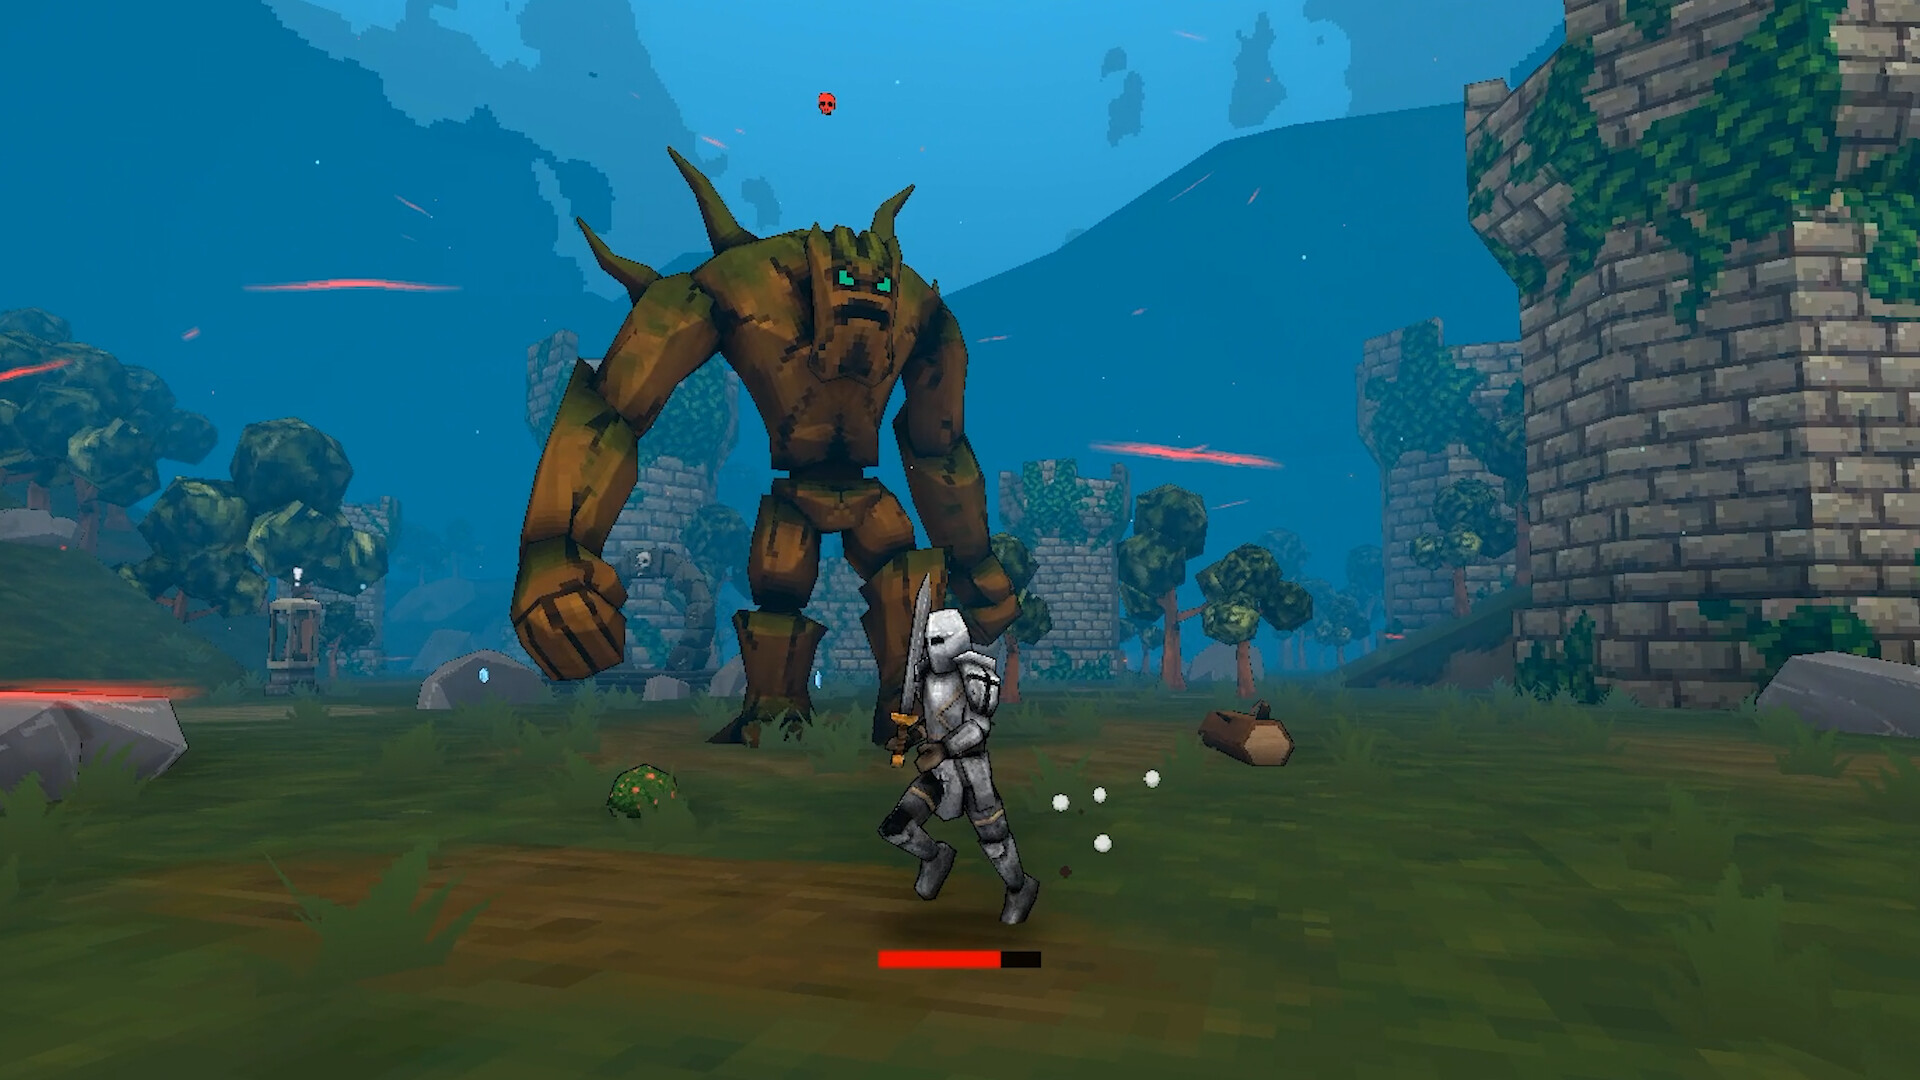
\includegraphics[width=0.5\textwidth]{megabonk.jpg}
    \caption{Megabonk Retro Style graphics}
    \label{fig:yourlabel}
\end{figure}
\clearpage

\section{Specification}

\subsection{Game Story}
Claybound is set in the forgotten dungeon of a wizard unnamed, this chaotic basement is full of remnants of 
failed experiments, escaped creatures and magical neglect. Rather than clean it himself, the wizard decides to delegate this task. Using a hastily put together
spell, he created a clay humanoid called a homunculus and drop it into his dungeon with nothing but a basic weapon and vague instructions to sort everything out.
\newline
\newline 
The homunculus has no memory, no name and no choice. Armed with instinct and a range of scavenged items, the player must fight through waves of the dunegons inhabitants, locate the portal
to the next floor and defeat whatever the wizard left locked in the basement.
\subsection{Game aesthetics}
The overall aesthetic of the game is darkly comedic, the homuculus is an unwilling protagonist thrust into a dangerous situation, and the world reflects this. Enemies include failed experiments and escaped subjects. The story is mainly told environmentally rather than through cutscenes, thus rewarding players who interact 
throught the world with the dice roll system.
\subsection{Game content}
\subsection{Game mechanics}
\subsection{Game technology}

\clearpage

\section{Prototype}
\clearpage
\section{Conclusion}
\clearpage


\bibliography{references}

\appendix
\clearpage

\section{Appendix}
\subsection{System Architecture}
\label{app:architecture}



\clearpage






\end{document}

